\documentclass[12pt,a4paper]{article}
\usepackage{datetime} 
\usepackage[T1]{fontenc}
\usepackage[utf8]{inputenc}
\usepackage{graphicx} 
\usepackage{url}
\graphicspath{{images/}} 
\usepackage{hyperref}
\usepackage{amsmath}
\renewcommand{\figurename}
\newline

\title
{\bf\fontsize{12pt}{14pt}
\selectfont KÜTAHYA SAĞLIK BİLİMLERİ ÜNİVERSİTESİ \\ MÜHENDİSLİK VE DOĞA BİLİMLERİ FAKÜLTESİ}

\date{}

\begin{document}

	
\maketitle

\begin{center}
	
\includegraphics{ksbu.png}
\end{center}

\begin{center}
	\vspace{1cm} 
\end{center}

\begin{center}
	\title
 {\bf\fontsize{12pt}{14pt}
 \selectfont YAPAY ZEKA DERSİ }
\end{center}

\begin{center}
		\title
  {\bf\fontsize{12pt}{14pt}
  \selectfont Yapay Arı Kolonisi Temelli Veri Madenciliği Algoritmalarının Geliştirilmesi ve Analizi}
\end{center}

\begin{center}
	\vspace{1cm} 
\end{center}

\begin{center}
		
\author
{\bf\fontsize{12pt}{14pt}HASAN GÖÇER\hspace{1.5cm}2118121021}
 
    \begin{center}
	   \vspace{1cm} 
    \end{center}
\date{\today} 
\end{center}


\begin{document}
\maketitle
\newpage
\begin{abstract}
Son yıllarda, araştırmacılar sosyal böceklerin davranışlarını inceleyerek sürü zekası kavramını kullanmaya başladılar ve bu sayede yapay sistemler geliştirdiler. Bu alanda yapay arı koloni optimizasyonu gibi algoritmalar ön plana çıktı. Yapılan çalışmalar, yapay arı kolonisi optimizasyonunun diğer sürü zekası algoritmalarına göre daha doğru sonuçlar verdiğini gösteriyor. Bu çalışma, veri madenciliği problemlerini çözmek amacıyla yapay arı algoritması (YAK) tabanlı veri madenciliği algoritmalarını geliştirmeyi hedeflemektedir. YAK algoritmasını analiz edip, paralel Yapay Arı Kolonisi algoritması geliştirilerek hızlandırma denendi. Ayrıca, Yapay Arı Kolonisi-tabanlı sınıflandırma algoritmaları ve işbirlikçi Yapay Arı Kolonisi-tabanlı sınıflandırma algoritmaları da çeşitli veri madenciliği sınıflandırma problemlerine uygulandı.
\end{abstract}

\section*{Anahtar Kelimeler}
Yapay Arı Kolonisi, Veri Madenciliği, Optimizasyon Algoritmaları, Sürü Zekası, Yapay Zeka,Particle Swarm Optimization Algoritmaları, Harris Hawks Optimization Algoritmaları,Differential Evolution  Algoritmaları,Gravitational search Algoritmaları

\section{Giriş/Amaç}
Bu çalışma, yapay arı kolonisi temelli optimizasyon algoritmalarının veri madenciliği problemlerine uygulanmasını amaçlamaktadır. Literatürdeki eksiklikler ve mevcut arı algoritmalarının sınırlılıkları üzerinde durulacak ve önerilen Yapay Arı Kolonisi tabanlı algoritmaların performansı gösterilecektir.

Yapay arı kolonisi algoritmaları, gerçek arı kolonilerinin davranışlarını taklit ederek problem çözme yetenekleri üzerine kuruludur. Bu algoritmalar, kaynak tahsisi, veri kümeleme, örüntü tanıma ve diğer veri madenciliği problemlerinde kullanılabilir. Ancak mevcut arı algoritmalarının bazı sınırlılıkları bulunmaktadır. Örneğin, bazı algoritmaların yakınsama hızı düşük olabilir veya çeşitli problem tipleri için yeterince genelleştirilemezler.

Bu çalışmada, literatürdeki eksiklikler ve mevcut arı algoritmalarının sınırlılıkları detaylı bir şekilde incelenecektir. Ardından, bu sınırlılıkları gidermek ve performansı artırmak amacıyla yeni yapay arı kolonisi tabanlı algoritmalar önerilecektir. Bu algoritmaların, farklı veri madenciliği problemlerindeki performansı deneysel olarak gösterilecek ve karşılaştırmalı analizler yapılacaktır.

\section{Literatür Araştırması}
Arı algoritmalarının teorisi ve uygulama alanları geniş bir çerçevede incelenmiş, ancak özellikle çok boyutlu problemlerin çözümünde bazı sınırlılıklar tespit edilmiştir. Yapay arı kolonisi algoritmaları büyük veri kümeleri üzerinde düşük performans sergilemiştir. Diğer sezgisel algoritmalarla karşılaştırıldığında belirli sınırlılıklar ortaya çıkmıştır.


\section{Yöntem}
Çalışmada, Yapay Arı Kolonisi algoritması ve türevleri olan paralel Yapay Arı Kolonisi  algoritması, Yapay Arı Kolonisi tabanlı sınıflandırma algoritmaları ve işbirlikçi Yapay Arı Kolonisi-tabanlı sınıflandırma algoritmaları kullanılmıştır. Bu yöntemler veri madenciliği problemlerine uygulanmış ve performansları ölçülmüştür.
\cite{ahmetcevahircinar}

\item
 {\bf\fontsize{12pt}{14pt}\selectfont
 Yapay Arı Kolonisi Nedir ve Arı çeşitleri Nelerdir ?}
 \newline\newline

 Yapay Arı Kolonisi Algoritması (YAK), Derviş Karaboğa tarafından arıların grup olarak yiyecek arama sürecinde sergiledikleri davranışları temel alınarak geliştirilmiş bir optimizasyon algoritmasıdır. Bu algoritmanın temelinde, topluluk halinde yemek arayan arıların bu süreçte izledikleri yol ve yöntemlerin incelenerek elde edilen sonuçların, optimizasyon problemlerinin giderilmesinde kullanılması sağlanıyor. Kovan da 3 çeşit arı vardır. Bunlar kraliçe arı, erkek arı ve dişi arıdır.

 Kaşif Arı : Belirli alandaki rastgele kaynaklar hakkında çeşitli bilgi toplar ve kovana nektar örneği taşır. Sonrasında görevi değişebilir.
 
Gözcü Arı : Kovanda beklerken dans alanını takip eden, uygunluk derecesine göre besin kaynağına yönelen arılardır.

İşçi Arı : Nektar taşımakla görevli olan arılardır. 



\item
{\bf\fontsize{12pt}{14pt}
\selectfont Yapay Arı Kolonisinin Rastrigin Fonksiyonu İle Matematiksel Gösterimi} \newline
1) Yapay Arı Kolonisi Algoritması (YAK), besin kaynaklarını içeren bir kovan çevresini temsil eder ve bu alanda optimal çözümleri arar. İlk aşamada, rastgele yiyecek kaynakları üretmek için bir süreç gereklidir. Bu süreç, her bir parametrenin belirlenen alt ve üst sınırları arasında rastgele değerler üreterek gerçekleştirilir. Bu adım, algoritmanın başlangıç noktasını oluşturur ve ardından yapay arılar, bu başlangıç kaynakları etrafında toplanarak optimize edilmiş çözümler aramaya başlarlar.
\begin{equation}
    X = X_{min_j} + rand(0, 1) \cdot (X_{max} - X_{min_j}) \quad (1) 
\end{equation}
Burada i=1… SN, J=1…D ve SN yiyecek kaynağı sayısı ve D is optimize edilecek parametre sayısıdır. Xmin j parametrelerin alt sınırıdır.

\newline

2) Her bir yiyecek kaynağının bir işçi arısı tarafından görevlendirildiği Yapay Arı Kolonisi Algoritması'nda, her kaynağın bir işçi arısıyla eşleştiği belirtilmiştir. İşçi arılar, çalıştıkları yiyecek kaynağı komşuluğunda yeni bir kaynak belirler ve bu kaynağın kalitesini değerlendirirler. Eğer yeni kaynak daha iyiyse, işçi arı bu yeni kaynağı hafızasına alır. Bu süreç, mevcut kaynağın komşuluk bölgesinde yeni bir kaynağın belirlenmesini temsil eder.
\begin{equation}
 V_{ij} = X_{ij} + Q_{ij}(X_{min_ij}-X_{kj}) (2)  
\end{equation}

Her bir kaynak için, çözümünün (xi) bir parametresi (rastgele seçilen j) değiştirilerek xi komşuluğunda yeni bir çözüm (vi) bulunur. Bu işlemde, j parametresi rastgele [1, D] aralığında bir tamsayı olarak seçilir. Yeni çözüm bulunurken, mevcut kaynağın j parametresi ile bir başka rastgele seçilen komsu çözümün j parametresi arasındaki fark alınır. Bu fark, [-1, 1] arasında rastgele değer alacak şekilde ağırlanır ve mevcut kaynağın j parametresine eklenir.

Bu işlemde, çözümler birbirine benzerse xi'nin j parametresindeki değişim miktarı azalır. Böylece, bölgesel optimal çözüme yaklaşıldıkça değişim miktarı adaptif olarak azalır.

Elde edilen yeni çözümün parametre değerleri, önceden belirlenen parametre sınırlarını aşarsa, ilgili parametrenin alt veya üst sınır değerlerine ötelenir.

\begin{equation}
V_{ij} = \left\{
\begin{aligned}
x_j^{mi^n} &\quad \text{if} \quad V_{ij} < x_j^{mi^n} \\  (3)
x_j^{min} &\leq V_{ij} \leq x_j^{max}  \\
x_j^{max} &\quad \text{if} \quad V_{ij} > x_j^{max}
\end{aligned}
\right\}

\end{equation}
Sınırlar dâhilinde üretilen vi parametre vektörü yeni bir kaynağa temsil etmekte ve bunun kalitesi hesaplanarak bir uygunluk değeri atanmaktadır (Eşitlik-4).
\begin{equation}
\text{fitness} =
\begin{cases}
\frac{1}{1+f_i} &  f_i \geq 0 \\
\frac{1}{|\text{abs}(f_i)|} & f_i < 0    (4) 
\end{cases}
\end{equation}

Burada, fi ve vi kaynaklarının (çözümlerinin) maliyet değerleri olarak tanımlandığını belirtmek gerekir. xi ve vi çözümleri arasında nektar miktarlarına (uygunluk değerlerine) göre açgözlü bir işlem uygulanır. Yeni bulunan vi çözümü, daha iyi ise, görevli arı eski kaynağın yerini silerek vi kaynağını hafızaya alır. Eğer yeni çözüm iyileşme göstermezse, görevli arı xi kaynağına devam eder ve xi çözümü geliştirilemediği için geliştirememe sayacı (failure) bir artar. Ancak xi çözümü geliştirildiğinde, sayaç sıfırlanır. Bu süreçte, en iyi çözümler arasında geçiş yapılırken açgözlü bir strateji izlenir.


3) Görevli arılar bir çevrimde araştırmalarını tamamladıktan sonra buldukları kaynakların nektar miktarlarıyla ilgili bilgiyi gözcü arılara aktarırlar. Gözcü arılar, dans aracılığıyla paylaşılan bilgiden faydalanarak yiyecek kaynaklarının nektar miktarlarına orantılı bir olasılıkla bir bölgeyi seçerler. Bu, Algoritma Yapay Arı Kolonisi'nin (ABC) çoklu etkileşim sergilediği bir örnektir. Olasılıksal seçme işlemi, uygunluk değerlerine dayanarak yapılır. Temel ABC algoritmasında bu seleksiyon işlemi rulet tekerleği kullanılarak gerçekleştirilir. Rulet tekerindeki her dilimin açısı, uygunluk değeri toplamına oranlanarak o kaynağın diğer kaynaklara göre nispi seçilme olasılığını belirtir.

\begin{equation}
p_{i} = \frac{fimess_{i}}{\sum_{i=1}^{SN} fimess_{i}} (5) 
\end{equation}
Burada  kaynağın kalitesini SN görevli arı sayısını göstermektedir. Bu olasılık hesaplama işlemine göre bir kaynağın nektar miktarı arttıkça (uygunluk değeri arttıkça) bu kaynak bölgesini seçecek gözcü arı sayısı da artacaktır. Bu özellik ABC’ nin pozitif geri besleme özelliğine karşılık gelmektedir.

\newline

4) Olasılık değerleri hesaplandıktan sonra, her bir kaynak için [0,1] aralığında rastgele bir sayı üretilir ve bu değer pi'den büyükse (pi, üretilen rastgele sayı), gözcü arılar görevli arılar gibi Eşitlik-2'yi kullanarak bu kaynak bölgesinde yeni bir çözüm üretir. Yeni çözüm değerlendirilir ve kalitesi hesaplanır. Ardından, yeni çözümle eski çözümün uygunluk değerleri karşılaştırılarak en iyi olan seçilir, açgözlü seleksiyon işlemine tabi tutulur.

Eğer yeni çözüm daha iyiyse, eski çözüm yerine bu çözüm alınır ve çözüm geliştirememe sayacı (failure) sıfırlanır. Eski çözümün uygunluğu daha iyi ise, bu çözüm muhafaza edilir ve çözüm geliştirememe sayacı bir artırılır. Bu süreç, tüm gözcü arılar yiyecek kaynağı bölgelerine dağılana kadar devam eder.

\newline

5) Bir çevrimin sonunda, tüm görevli ve gözcü arılar arama süreçlerini tamamlar ve çözüm geliştirememe sayaçları kontrol edilir. Bir arının bir kaynağı terk edip etmediği, yani gidip geldiği kaynağın nektarının tükenip tükenmediği, çözüm geliştirememe sayaçları aracılığıyla belirlenir. Bir kaynak için çözüm geliştirememe sayacı belli bir eşik değerinin üzerindeyse, bu kaynağın görevli arısının tükenmiş olan çözümü bırakıp kendisi için başka bir çözüm araması gerekir. Bu durumda, kaynakla ilişkili görevli arı, kaşif arıya dönüşür ve rastgele çözüm arama süreci başlar. Bu dönüşüm için kullanılan eşik değeri ABC algoritmasının önemli bir kontrol parametresidir ve "limit" olarak adlandırılır. Temel ABC algoritmasında, her çevrimde yalnızca bir kaşif arının çıkmasına izin verilir.

Bu süreç, görevli ve gözcü arıların arama süreçlerini tamamladıktan sonra, çözüm geliştirememe sayaçlarının kontrol edilmesiyle başlar. Ardından, tükenmiş kaynaklarla ilişkili görevli arılar kaşif arıya dönüşür ve yeni bir çözüm arama süreci başlatılır. Bu döngü, ABC algoritmasının önemli bir parçasını oluşturur ve Şekil-3'te gösterilen akış diyagramıyla görselleştirilebilir.
\cite{emoek}
\cite{emo}
\item

{\bf\fontsize{12pt}{14pt}
\selectfont Yapay Arı Kolonisine Benzer Optimizasyon Algoritmaları} \newline

1-) Particle Swarm Optimization Algorithm (PSO) \newline
2-) Harris Hawks Optimization Algorithm (HHO) \newline
3-) Differential Evolution  Algorithm (DE) \newline
4-) Gravitational search Algorithm (GSA) \newline

{\bf\fontsize{12pt}{13pt}
1-) Particle Swarm Optimization Algorithm (PSO)}
PSO (Particle Swarm Optimization) algoritması, optimizasyon problemlerinde kullanılan bir meta-sezgisel yaklaşımdır. Algoritmanın temel çalışma prensibi, çoklu parçacıkların rastgele başlangıç konumları ve hızlarıyla birlikte bir çözüm uzayında hareket etmeleridir. Her parçacık, problemdeki bir çözümü temsil eder ve en iyi konumlarına (kişisel en iyi) ve tüm parçacıklar arasındaki en iyi konuma (küresel en iyi) doğru hareket eder.

Parçacıklar, mevcut konumları ve hızlarıyla birlikte en iyi konumlarına doğru güncellenir. Bu güncellemeler, parçacıkların hareket yönünü ve hızını dengeleyerek mevcut en iyi konumlar doğrultusunda gerçekleşir. Algoritma belirli bir iterasyon sayısına veya konverjans kriterine ulaşana kadar parçacıkların konumlarını ve hızlarını günceller. Sonuç olarak elde edilen konumlar, problemdeki optimum çözümü temsil eder.

PSO, genellikle gerçek sayılarla ifade edilen optimizasyon problemleri için kullanılır ve çok boyutlu, karmaşık uzaylarda etkilidir. Popülasyon tabanlı bir yaklaşım olan PSO, çeşitli optimizasyon problemlerinde başarılı sonuçlar verir ve kolayca uygulanabilir bir algoritmadır.


{\bf\fontsize{12pt}{13pt}
2-) Harris Hawks Optimization Algorithm (HHO)}
Harris Hawks Optimizasyonu (HHO), doğal olarak Harris şahinlerinin avlanma stratejilerinden ilham alan bir optimizasyon algoritmasıdır. Bu algoritma, bir problemde en iyi çözümü bulmak için doğal süreçleri taklit eder. HHO, grup içinde işbirliği yaparak ve en iyi çözüme odaklanarak çözüm uzayını araştırır. Temel adımları arasında rastgele çözüm üretme, çözümleri değerlendirme ve yeni çözümler üretme yer alır. Yerel ve küresel arama stratejilerini birleştirerek karmaşık optimizasyon problemlerinde etkili bir alternatif sunar.


{\bf\fontsize{12pt}{13pt}
3-) Differential Evolution  Algorithm (DE)}
Differential Evolution (DE), evrimsel optimizasyon temelli bir algoritmadır. Bir fonksiyonun en iyi değerini bulmak için kullanılır. DE, bir popülasyon içindeki bireyler arasında çaprazlama ve mutasyon işlemleri uygulayarak yeni bireyler üretir. Bu yeni bireyler arasından en iyi olanlar seçilerek popülasyon güncellenir. Algoritma, karmaşık optimizasyon problemleri için kullanışlıdır ve genellikle diğer optimizasyon yöntemlerinden daha az parametre kullanır.

 \begin{figure}[h] % Resmin konumunu belirtmek için kullanılır (h: burada, t: sayfanın en üstü, b: sayfanın en altı, ...)
    \centering
    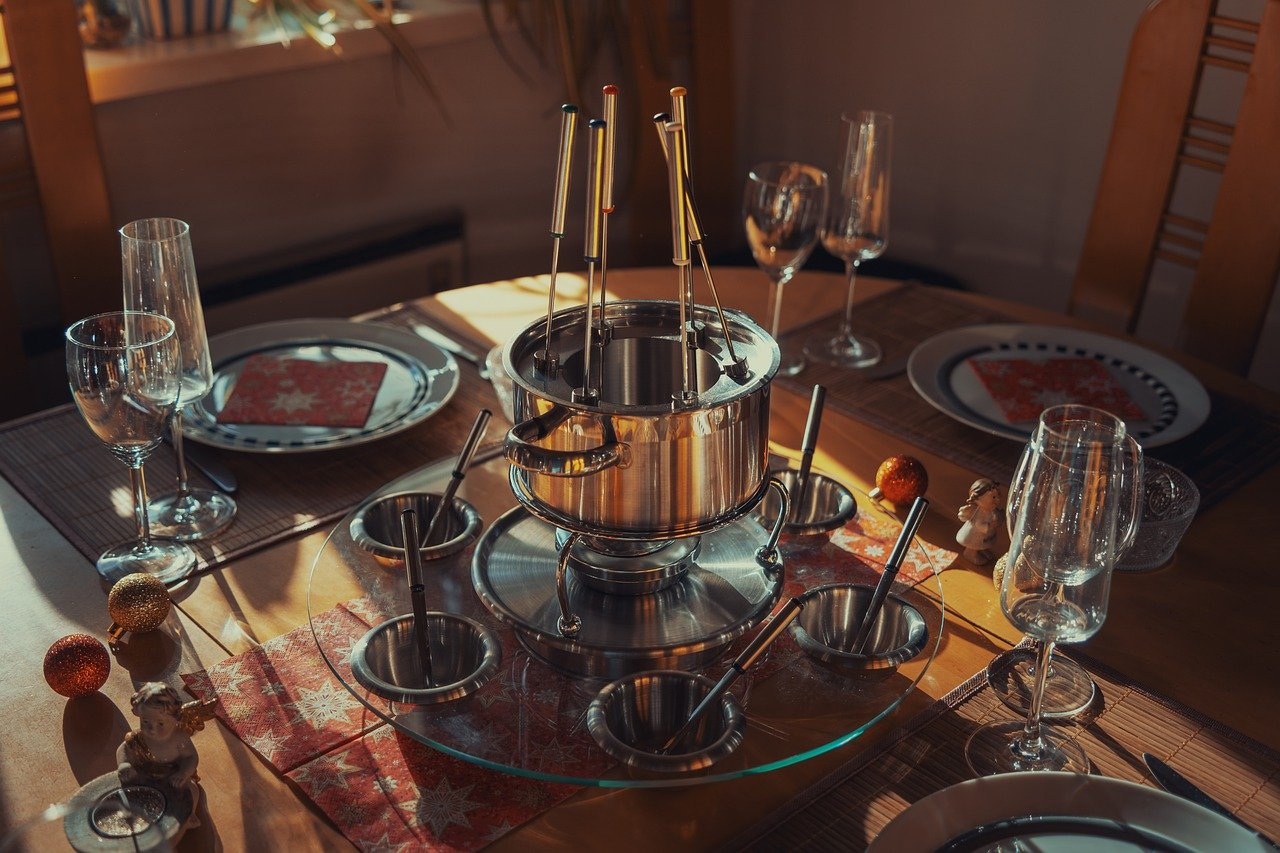
\includegraphics[width=0.5\textwidth]{100.png} % PNG dosyasının yolu ve dosya adı
    \caption{Diferansiyel Gelişim Algoritması } % Resmin altında gösterilecek açıklama metni
\end{figure}

\begin{itemize}
    \item NP : populasyon büyüklüğü (kromozom sayısı) NP ≥4 (1, 2, 3, …, i)
    \item D : değişken sayısı (gen sayısı) (1, 2, 3, …, j)
    \item CR : çaprazlama oranı [0.1,1.0]
    \item G : jenerasyon (1, 2, 3, …, Gmax)
    \item F : ölçekleme faktörü 
    \item \verb|XjiG| : G jenerasyonunda, i kromozomunun j parametresi (gen)
    \item  \verb| nj,i,G+1| : mutasyon ve çaprazlamaya tabi tutulmuş ara kromozom
    \item \verb|uj,i,G+1 | : uj,i,G+1 : xj,i,G den bir sonraki jenerasyon için üretilen kromozom (child-trial) 
    \item \verb|r1,2,3 | : yeni kromozomun üretilmesinde kullanılacak rasgele seçilmiş kromozomlar
\end{itemize}

Probleme ait değişken sayısı D, her bir kromozomun içerdiği gen sayısını belirler. NP ise kullanıcı tarafından belirlenen kromozom sayısıdır. NP her zaman üçten büyük olmalıdır; çünkü Genetik Algoritmalar (DGA) kullanılarak yeni kromozomların üretilmesi için mevcut kromozomların dışında en az üç adet kromozoma ihtiyaç duyulur .


{\bf\fontsize{12pt}{13pt}\selectfont Mutasyon }\newline
Mevcut kromozomun belirli genlerinde rasgele değişiklikler yaparak çözüm uzayında hareket etmesini sağlar. Doğru mutasyon işlemi için, diferansiyel gelişim algoritmasında kullanılan kromozomların belirli bir yönde ve miktarda değişmesi gerekir.

Diferansiyel gelişim algoritmasında, mutasyona uğrayacak kromozom dışında, birbirinden farklı üç kromozom seçilir (r1, r2, r3). Seçilen ilk iki kromozom arasındaki fark alınır. Ardından bu fark, bir ağırlık parametresi F ile çarpılır. F genellikle 0 ile 2 arasında değer alır. Elde edilen ağırlıklı fark, üçüncü seçilen kromozom (r3) ile toplanarak, yeni bir mutasyona uğramış kromozom elde edilir. Bu işlem sonucunda elde edilen kromozom, çaprazlama işlemi için kullanılır.


{\bf\fontsize{12pt}{13pt}\selectfont Çaprazlama }\newline  
Çaprazlama işlemi, mutasyon sonucu elde edilen farklı kromozom ile mevcut kromozomun birleştirilerek yeni bir deneme kromozomu üretme sürecidir. Yeni kromozom oluşturulurken her gen için belirli bir olasılıkla farklı kromozomdan gen seçilirken, geri kalan genler mevcut kromozomdan alınır. Bu yöntem, belirli bir çaprazlama oranı (CR) ile düzenli çaprazlama yönteminin (uniform crossover) geliştirilmiş halidir. Amaç, yeni kromozomda belirli oranda genin farklı kromozomdan alınmasını sağlamaktır.


{\bf\fontsize{12pt}{13pt}\selectfont Seçim }\newline 
Yeni jenerasyonun oluşturulması için, seçim operatörü kullanılarak mevcut jenerasyondan ve üretilen yeni kromozomlardan oluşan bir grup değerlendirilir. Kromozomların yeni jenerasyonda yer alma olasılıkları, genellikle uygunluklarına (fitness) dayanır. DGA'da (Differansiyel Genetik Algoritmalar) karşılaştırma doğrudan yapılır, bu nedenle seçim için karmaşık operatörlere gerek duyulmaz. En yüksek uygunluk değerine sahip kromozomlar, yeni jenerasyonun üyeleri olarak seçilir ve atanır.

\newpage
{\bf\fontsize{12pt}{13pt}\selectfont Algoritmanın Durdurulması }\newline
Yeni jenerasyonlar, belirli operatörler kullanılarak oluşturuluyor. Temel amaç, her seferinde daha iyi uygunluk değerine sahip kromozomlar elde etmek ve en iyi çözüme yaklaşmaktır. Bu süreç, genellikle G = Gmax (maksimum iterasyon sayısı) olduğunda sonlandırılır. Ayrıca, algoritmanın durdurulması için populasyondaki en iyi ve en kötü uygunluk değerleri arasındaki farkın çok küçük bir seviyeye ulaşması da bir kriter olabilir.



{\bf\fontsize{12pt}{13pt}
4-) Gravitational search Algorithm (GSA)}
Gravitational Search Algorithm (GSA), doğa olaylarından esinlenerek geliştirilen bir optimizasyon algoritmasıdır. Maddenin çekim prensibini temel alır. Her çözüm adayını bir kütle olarak temsil eder ve bu kütleler arasındaki yerçekimi etkileşimini simüle ederek en iyi çözümü bulmaya çalışır. Büyük kütleler, daha güçlü çekim etkileriyle diğer kütleleri çeker ve böylece çözüm uzayında optimal bir çözüm bulunmaya çalışılır. GSA, karmaşık optimizasyon problemleri için kullanılan bir evrimsel hesaplama yöntemidir.
\cite{nuhazginoglu}
\cite{dergipark1095957}


\item 

\section{Bulgu ve Tartışma}
Veri madenciliği problemlerinde Yapay Arı Kolonisi temelli algoritmaların performansı incelenmiş, elde edilen sonuçlar literatürdeki diğer optimizasyon algoritmalarıyla karşılaştırılarak değerlendirilmiştir. Çeşitli ölçüm metrikleri kullanılarak algoritmaların etkinliği ve başarımı analiz edilmiştir.

\section{Sonuçlar}
Yapılan çalışmalar, önerilen Yapay Arı Kolonisi tabanlı algoritmaların veri madenciliği problemlerinde performansını artırdığını ve daha geniş bir problem yelpazesine uygulanabilirliğini sağladığını göstermektedir.

\section{Gelecekte Yapılacak Çalışmalar}
Gelecekte, Yapay Arı Kolonisi tabanlı algoritmalardan Differential Evolotion algoritması ile karşılaştırmalar yapılıp Differential Evolotion algoritmasının kodları incelenecek ve Differential Evolotion algoritması hakkında detaylı bilgi sahibi olunacaktır .

\newpage

\bibliographystyle{plain}
\bibliography{references}

\end{document}